\chapter{Introduction}
\label{chapter:introduction}

As neuromorphic computing regularly becomes a popular scientific topic, various  applications for such systems emerge and make use of advantages that analogue hardware has over traditional computers \reference{paper on current neuromorphic computing}.
In order to do this, one must get familiar with the system that is used as it often differs in many ways from common computer architectures.
Thus programing for such systems can feel odd at times as users need to abandon some familiar techniques and acquire new skills instead.
This is a hurdle for many users when developing new experiments and initially takes a significant amount of time. 
\\
\\
An example of this is the current way of programming for the plasticity processing unit of the \ac{HICANN-DLS}. 
The \ac{HICANN-DLS} is a small scale system that features analogue emulation of neurons and synapses in networks.
The \ac{PPU}, as part of \ac{HICANN-DLS}, can be used for implementing plasticity rules for such networks.
It resembles a processor architecture which was modified for this task.
Implementing such plasticity rules differs from conventional high-level programming styles. 
When creating code for the \ac{PPU}, users are pretty much pushed back to the origins of computing;
Instead of assigning values like |d = a + b|, one must first read the variables from memory, then operate on their values and finally write back the result to memory.
Therefore coding for the \ac{PPU} works on a low level which brings its own challenges to the user.

Ultimately, the more a system abandons conventional elements of programming, the more problems can emerge from this.
Not only will fewer users take the initiative of writing code for such systems, but also can code get confusing, hard to debug and at worst even inefficient.
\\
\\
Compilers usually save users from these problems by offering high-level languages
Over decades compilers have been developed and became standard tool for programmers.
At the same time compilers became more and more a black box that transforms a program into an executable file.
For this reason it may be difficult for some users to abandon their convenience and go back to low-level programming.

Though the \ac{PPU} is not completely without compiler support, its distinct features are only usable on a low level.
As these features are necessary to implement plasticity rules on the \ac{HICANN-DLS} this can easily cause inconveniences for users.
Users repeatedly mix high-level and low-level programming which is an atypical style of programming.
It can lead to different problems as users have to adapt to this and at worst this can even lead to ineffective programs.
As performance is important for neuromorphic programming, users may need an unreasonable amount of time and work to achieve simple results with this.
\\
\begin{wrapfigure}{R}{0.4\textwidth}
\captionsetup{format=plain, indention=.6cm, labelsep=newline,singlelinecheck=false}
    \centering
    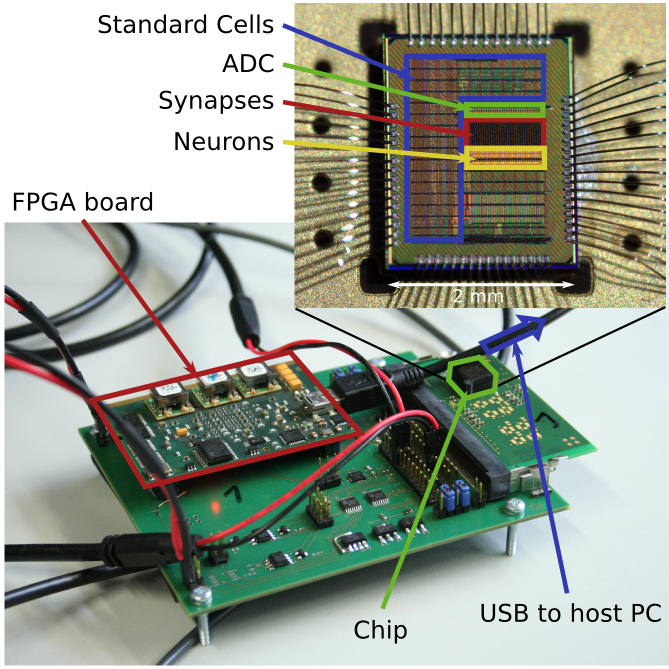
\includegraphics[width=0.4\textwidth]{pictures/Fig1.png}
    \caption{\label{fig:dlsboard} Set-Up of a \ac{HICANN-DLS} Test System (from \citeauthor{PPU})}
\end{wrapfigure}
\\
Full compiler support doe not exist for the \ac{PPU} because of its modified processor architecture, which was developed solely for neuromorphic hardware.
It can be classified as an application specific instruction set architecture which is an intermediate form between general purpose processors and application specific integrated circuits.
It offers a partly customized instruction set that is optimized for its applications.
\\
\\
The \ac{HICANN-DLS} already is an experimental platform, which is used by several users, even though of \ac{PPU}-related challenges.
Applications like in-the-loop training or stimulated time dependent plasticity have been developed and mostly do not involve the \ac{PPU} .
Even when taking the effort of learning to code for the \ac{PPU}, users are constantly challenged by missing programming features such as creating parameterized functions.
This leads to repetitive code or difficulties when involving calibration into code.

Offering more tools for the \ac{PPU} could reduce the effort of developing for the \ac{PPU}, while at the same time increasing capabilities of programs.
Besides allowing full high-level programming, compiler support could also offer tools like code optimization and debugging features.
This work therefore aims to achieve compiler support for the \ac{PPU}'s hardware with as many features as possible.
At some point compiler support may also facilitate automatic code generation as a prerequisite for implementation of very high-level languages.
Users then could create plasticity rules in existing program environments from where code is translated into \ac{PPU} programs.
This creates the need for optimization of \ac{PPU} code, like those built into virtually every compiler.
\\
\\
This thesis will focus on achieving aforementioned compiler support and briefly explain the process itself.
As fundamental knowledge of both processors and compilers is needed along the way, the second chapter will start with a very basic introduction to both topics.
This involves basic information for the \ac{PPU} as well as \ac{GCC} and should explain the basic concepts to an extend which is sufficient.
Afterwards, the process of extending the compiler is explained, followed by a presentation of results as well as first test cases.
The thesis will conclude in a resume and give an outlook to future applications and development of the compiler and the \ac{PPU}.

Ultimately this work wants to simplify \ac{PPU} programming overall and give users tools at hand that allow for novel experiments and encourage further development of the whole system.




